\subsection{Build the Blink sample application}
This quickstart shows how to enable application development on an Azure Sphere device and how to build and debug a sample application. It uses the Blink sample, which is part of the Azure Sphere SDK. The Blink sample shows how to access GPIOs and LEDs on the development board.

This section requires:
\begin{itemize}
    \item Your Azure Sphere device is connected to your PC
    \item You have completed all the steps to \autoref{sec:install}
\end{itemize}

\subsubsection{Prepare your device for development and debugging}
By default, Azure Sphere devices are "locked", which is they do not allow applications to be loaded or debugging on the board from a PC.

The azsphere device prep-debug command configures the device to accept applications from a PC for debugging and loads the debugging server onto the device. It also assigns the device to a device group that does not allow over-the-air (OTA) application updates. During application development and debugging, you should leave the device in this group so that OTA application updates do not overwrite the application under development.

To prepare your device:
\begin{enumerate}
    \item Make sure that your Azure Sphere device is connected to your PC, and your PC is connected to the internet.
    \item In an Azure Sphere Developer Command Prompt window, type the following command:
    \begin{lstlisting}[language=bash]
    azsphere device prep-debug
    \end{lstlisting}
    
    You should see output similar to the following:
    \begin{lstlisting}[]
    Getting device capability configuration for application development.
    Downloading device capability configuration for device ID 'B3E012CE682BA0A6235866AB3A87D838A4817E5C539832A34BF7A715CA8D015FF99C84B909CB2886916259AD186B212E148FC9C4BF8BB6A275A11A2B9495D578'.
    Successfully downloaded device capability configuration.
    Successfully wrote device capability configuration file 'C:\Users\A548068\AppData\Local\Temp\tmpCCF6.tmp'.
    Setting device group ID 'cd037ae5-27ca-4a13-9e3b-2a9d87f9d7bd' for device with ID 'B3E012CE682BA0A6235866AB3A87D838A4817E5C539832A34BF7A715CA8D015FF99C84B909CB2886916259AD186B212E148FC9C4BF8BB6A275A11A2B9495D578'.
    Successfully disabled over-the-air updates.
    Enabling application development capability on attached device.
    Applying device capability configuration to device.
    Successfully applied device capability configuration to device.
    The device is rebooting.
    Installing debugging server to device.
    Deploying 'C:\Program Files (x86)\Microsoft Azure Sphere SDK\DebugTools\gdbserver.imagepackage' to the attached device.
    Image package 'C:\Program Files (x86)\Microsoft Azure Sphere SDK\DebugTools\gdbserver.imagepackage' has been deployed to the attached device.
    Application development capability enabled.
    Successfully set up device 'B3E012CE682BA0A6235866AB3A87D838A4817E5C539832A34BF7A715CA8D015FF99C84B909CB2886916259AD186B212E148FC9C4BF8BB6A275A11A2B9495D578' for application development, and disabled over-the-air updates.
    Command completed successfully in 00:00:41.4376552.
    \end{lstlisting}
\end{enumerate}

\subsubsection{Build and run the Blink sample}
\begin{enumerate}
    \item Start \textbf{Visual Studio 2017} and go to \textbf{File>New>Project}. The templates for the Azure Sphere are available in \textbf{Visual C++>Cross Platform>Azure Sphere}. Select \textbf{Blink Sample for MT3260 RDB(Azure Sphere)}.
    
    \item Enter a name and location for the project, or you can just click OK in default name and location.
    
    \item Open the main.c in the \textbf{Solution Explorer>Source Files}, if you cannot see the \textbf{Solution Explorer} you can find it in \textbf{View>Solution Explorer}. Navigate to the line that tests the value of newButtonState and press F9 to set a breakpoint:
    \begin{lstlisting}[language=c]
    if (newButtonState == GPIO_Value_Low) {
    \end{lstlisting}
    
    \item Ensure that your board is connected to your PC by USB. Then select \textbf{Remote GDB Debugger} from the menu bar or press F5.
    \begin{figure}[h]
        \centering
        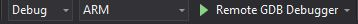
\includegraphics[scale=0.8]{VSDebug.JPG}
    \end{figure}
    
    \item If Visual Studio prompt to build the project, select Yes, it will creates an image package, sideloads it onto the board, and starts it in debug mode. Sideloading means the application is delivered directly from the PC over a wired connection, rather than delivered over the air(OTA) by Wi-Fi.
    \tcbset{colback=green!26}
    \begin{tcolorbox}
    \textsc{Tip \newline\newline Note the path in the Build output, which indicates the location of the output image package on your PC. You'll use the image package later for the deploy over Wi-Fi}
    \end{tcolorbox}
    
    \item Press button A. Visual Studio stops at the breakpoint that you set. Open \textbf{Debug>Windows} and select Autos to display the variables that are used in the current and previous statements. You should see the values like:
        \begin{figure}[h]
            \centering
            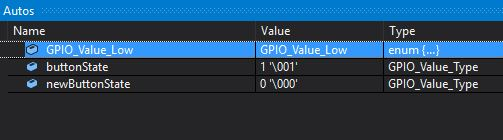
\includegraphics[scale=0.7]{BlinkDebugAuto.JPG}
        \end{figure}
    
    \item Select \textbf{Continue} in the menu bar. Execution pauses again at this breakpoint. Now the value of newButtonState variable is 1, which indicates a button release. Press F9 to remove the breakpoint. Then select \textbf{Continue}. Now, each time press and release Button A, the blink rate changes.
    
    \item To see the messages from the debugger, select \textbf{Debug>Windows>Output} in the dropdown menu.
    
    \item When you are done debugging, select the Stop icon in the menu bar or press Shift+F5.
\end{enumerate}

\subsection{Deploy an application over the air}
This section shows how to create your first over-the-air(OTA) application deplolyment. OTA deployment delivers an application through a feed to the devices in a devices group that match the target stock-keeping unit for the feed.

This section requires:
\begin{itemize}
    \item Your Azure Sphere device is connected to your PC
    \item You have completed all the steps to \autoref{sec:install}
    \item You have completed the previous section and retained the image package for the application
\end{itemize}

\subsubsection{Prepare your device for OTA deployment}
Before you start the OTA deployment process, your Azure Sphere must be ready to accept OTA application updates which means "lock" the device and enable OTA update so that it able to be operated by the customer site. The \textbf{azsphere device prep-field} command is the simplest way to do this. This command:
\begin{itemize}
    \item Disables the ability for Visual Studio to load applications onto the device, so that only OTA applications can be loaded
    \item Assigns a new product SKU to the device
    \item Assigns the device to a new device group that enables OTA application updates
\end{itemize}

The \textbf{azsphere device prep-field} command works on the device that is connected to PC. It has the following form:
\begin{lstlisting}[language=bash]
azsphere device prep-field --newdevicegroupname <unique-dg-name> --newskuname <unique-sku-name>
\end{lstlisting}

The --newdevicegroupname flag specifies a name for the new device group that the command creates. All device groups created by this command support automatic OTA application updates. Supply a descriptive name that is unique among the device group names in your Azure Sphere tenant.

The --newskuname flag specifies a name for the new product SKU that the command creates. A product SKU identifies a model of the connected device that contains an Azure Sphere chip. Each SKU in an Azure Sphere tenant must have a unique name.

The Azure Sphere related to the device has created a device group named "AFSphereGroup" and a product SKU named "AFSphereProductSKU". The command created the group and SKU is:
\begin{lstlisting}[language=bash]
azsphere device prep-field --newdevicegroupname "AFSphereGroup" --newskuname "AFSphereProductSKU"

Removing applications from device.
Component 'e3c4a1ff-8456-49e4-a353-a76235e5136f' deleted or was not present beforehand.
Removing debugging server from device.
Component '8548b129-b16f-4f84-8dbe-d2c847862e78' deleted or was not present beforehand.
Successfully removed applications from device.
Locking device.
Downloading device capability configuration for device ID 'B3E012CE682BA0A6235866AB3A87D838A4817E5C539832A34BF7A715CA8D015FF99C84B909CB2886916259AD186B212E148FC9C4BF8BB6A275A11A2B9495D578'.
Successfully downloaded device capability configuration.
Applying device capability configuration to device.
Successfully applied device capability configuration to device.
The device is rebooting.
Successfully locked device.
Creating a new device group with name 'AFSphereGroup'.
Setting device group ID '5ece1a6b-44b8-40cb-b0e3-623dccd5bc6e' for device with ID 'B3E012CE682BA0A6235866AB3A87D838A4817E5C539832A34BF7A715CA8D015FF99C84B909CB2886916259AD186B212E148FC9C4BF8BB6A275A11A2B9495D578'.
\end{lstlisting}

You aren't required to create a new device group and SKU every time you prepare a device for field use. Typically, you would create one SKU for each product model, and one device group for each collection of devices that you want to update together. To assign the device to different device group use the following command format:
\begin{lstlisting}[language=bash]
azsphere device prep-field --devicegroupid <device-group-id>
\end{lstlisting}
For example, to change the group to AFSphereGroup which created previously, use group id 5ece1a6b-44b8-40cb-b0e3-623dccd5bc6e in the command.

\subsubsection{Link the device to a feed}
The next step is to link your device to a feed that delivers the Blink application. You must supply:
\begin{itemize}
    \item The ID of Azure Sphere OS feed on which the application depends
    \item The path to the image package file that Visual Studio created for the Blink application
    \item A name for the feed that will deliver the application
\end{itemize}

To link to a feed:

\begin{enumerate}
    \item Get the feed ID for the Retail Azure Sphere feed, which delivers the Azure Sphere OS.
    \begin{lstlisting}[language=bash]
    azsphere feed list
    Listing all feeds.
    Retrieved feeds:
    --> [3369f0e1-dedf-49ec-a602-2aa98669fd61] 'Retail Azure Sphere OS'
    --> [82bacf85-990d-4023-91c5-c6694a9fa5b4] 'Retail Evaluation Azure Sphere OS'
    Command completed successfully in 00:00:03.0017019.
    \end{lstlisting}
    Copy the ID of the Retail Azure Sphere OS feed to use in the next step.
    
    \item Issue the azsphere device link-feed command to create a feed and associate it with the Blink image package that you created previously.
    \begin{lstlisting}[language=bash]
    azsphere device link-feed --dependentfeedid 3369f0e1-dedf-49ec-a602-2aa98669fd61 --imagepath "C:\Users\A548068\Documents\AZure\Blink\Mt3620Blink1\Mt3620Blink1\bin\ARM\Debug\Mt3620Blink1.imagepackage" --newfeedname "Mt3620Blink1"
    \end{lstlisting}
    The --dependentfeedid flag supplies the ID of the Retail feed.
    
    The --imagepath flag provides the path to the image package file for the Blink application. The full path to the image file is displayed in the Visual Studio 2017 Build Output windows. The azsphere device link-feed command uploads the image package file to the Azure Sphere Security Service and creates an image set with a unique name.
    
    The --newfeedname flag provides a name for the feed that the command creates. Feed names must be unique in an Azure Sphere tenant, so specify a name that distinguishes this feed from any others.
    
    The outout could be:
    \begin{lstlisting}[language=bash]
    Getting the details for device with ID 'B3E012CE682BA0A6235866AB3A87D838A4817E5C539832A34BF7A715CA8D015FF99C84B909CB2886916259AD186B212E148FC9C4BF8BB6A275A11A2B9495D578'.
    Uploading image from file 'C:\Users\A548068\Documents\AZure\Blink\Mt3620Blink1\Mt3620Blink1\bin\ARM\Debug\Mt3620Blink1.imagepackage':
     --> Image ID:       215c72b6-7472-4337-80c8-da98ef536f39
     --> Component ID:   e3c4a1ff-8456-49e4-a353-a76235e5136f
     --> Component name: 'Mt3620Blink1'
    Removing temporary state for uploaded image.
    Create a new feed with name 'Mt3620Blink1'.
    Adding feed with ID '8354ecb2-5348-4582-9e0c-ae9fc055f3db' to device group with ID '5ece1a6b-44b8-40cb-b0e3-623dccd5bc6e'.
    Creating new image set with name 'ImageSet-Mt3620Blink1-2019.02.22-16.15.07+01:00' for images with these IDs: 215c72b6-7472-4337-80c8-da98ef536f39.
    Adding image set with ID 'e05f2494-a716-48cb-9f41-4d1e1e6fbb7a' to feed with ID '8354ecb2-5348-4582-9e0c-ae9fc055f3db'.
    Successfully linked device 'B3E012CE682BA0A6235866AB3A87D838A4817E5C539832A34BF7A715CA8D015FF99C84B909CB2886916259AD186B212E148FC9C4BF8BB6A275A11A2B9495D578' to feed with ID '8354ecb2-5348-4582-9e0c-ae9fc055f3db'.
    Command completed successfully in 00:00:28.3808069.
    \end{lstlisting}
    
    This command creates a feed that is linked to the device group to which the attached device belongs—that is, the "AFSphereGroup"  created earlier in this quickstart. It will deliver the "Mt3620Blink1" application to all Azure Sphere devices in the group whose product SKU is "AFSphereProductSKU".
\end{enumerate}

\subsection{Update a deployment}
Get the feed ID we created above:
\begin{lstlisting}[language=bash]
    azsphere feed list
    
    Listing all feeds.
    Retrieved feeds:
    --> [3369f0e1-dedf-49ec-a602-2aa98669fd61] 'Retail Azure Sphere OS'
    --> [82bacf85-990d-4023-91c5-c6694a9fa5b4] 'Retail Evaluation Azure Sphere OS'
    --> [8354ecb2-5348-4582-9e0c-ae9fc055f3db] 'Mt3620Blink1'
    Command completed successfully in 00:00:02.2268023.
\end{lstlisting}
Copy the ID of Mt3620Blink1 for the application update.

To update a feed with a new version of your application, use the azsphere component publish command. This command uploads a new image package, creates a new image set, and adds the new image set to an existing feed.

For example, the following command update the Blink Application to the feed just created named Mt3620Blink1:
\begin{lstlisting}[language=bash]
azsphere component publish --feedid 8354ecb2-5348-4582-9e0c-ae9fc055f3db --imagepath "C:\Users\A548068\Documents\AZure\Blink\Mt3620Blink1\Mt3620Blink1\bin\ARM\Debug\Mt3620Blink1.imagepackage" 
\end{lstlisting}
